\label{sec:exchange-design}
Đổi món là quy trình thay thế một đơn đã thanh toán trước khi pha chế, không phải khách tự hủy để nhận tiền. Khách mở liên kết hỗ trợ trên Order PAID, chọn lại món/size/topping qua menu và giỏ đổi riêng; backend báo giá, khách gửi lý do và quầy quyết định. Mở menu hoặc nhận báo giá không tự hoàn kho hay đóng đơn cũ.

\subsubsection{Dữ liệu yêu cầu và báo giá}
OrderExchange lưu sourceOrderId, replacementOrderId, items, reason, trạng thái, quyết định và version. Liên kết hai Order giữ được lịch sử trước/sau thay vì sửa trực tiếp các dòng món của đơn đã thu tiền. Unique(sourceOrderId, key) cùng requestHash bảo vệ gửi lặp yêu cầu.

quotedLines/quotedTotal lưu báo giá đã nhận khi yêu cầu được tạo. Frontend gửi expectedQuote để backend đối chiếu fingerprint của báo giá; nếu giá/trạng thái đổi trước lúc gửi, khách phải xem lại. Fingerprint là dấu vân tay đối chiếu dữ liệu, không phải chữ ký cổng thanh toán. Khi đã tạo yêu cầu, bước duyệt dùng thành tiền snapshot, tránh tính lại theo giá menu mới trong lúc khách chờ.

\begin{table}[htbp]\centering\small
\begin{tabularx}{\linewidth}{|p{.24\linewidth}|X|}\hline
\textbf{Trạng thái} & \textbf{Ý nghĩa và tác động}\\\hline
REQUESTED & Chờ quầy; đơn nguồn vẫn PAID và giữ nguyên liệu. Chặn chuyển PREPARING cho tới khi xử lý yêu cầu.\\\hline
APPROVED & Đã tạo đơn thay thế, chuyển credit và đóng đơn nguồn trong cùng transaction.\\\hline
REJECTED & Quầy từ chối, lưu ghi chú; giữ nguyên món và tiền của đơn nguồn.\\\hline
WITHDRAWN & Khách rút yêu cầu còn chờ bằng version; tiếp tục đơn nguồn.\\\hline
\end{tabularx}\caption{Vòng đời yêu cầu đổi món, độc lập vòng đời Order}
\end{table}

\subsubsection{Chuyển giá trị đã trả và thu chênh lệch}
Giá trị có thể chuyển bằng tổng Payment đã áp dụng của đơn nguồn cộng creditApplied đã chuyển vào đơn đó; backend kiểm bằng total của đơn nguồn trước khi duyệt. Credit là giá trị gắn với đơn thay thế, không phải số dư ví dùng tùy ý.

\begin{table}[htbp]\centering\small
\begin{tabularx}{\linewidth}{|X|c|c|c|}\hline
\textbf{Trường hợp} & \textbf{Tiền cũ} & \textbf{Món mới} & \textbf{Thu thêm}\\\hline
Đổi bằng giá & 45.000đ & 45.000đ & 0đ\\\hline
Đổi cao hơn & 45.000đ & 75.000đ & 30.000đ\\\hline
Đổi thấp hơn & 45.000đ & 40.000đ & Yêu cầu chọn lại\\\hline
\end{tabularx}\caption{Ví dụ credit và số tiền thu thêm khi đổi món}
\end{table}

Order mới giữ total bằng giá trị món, creditApplied bằng tiền chuyển, amountDue bằng phần chênh lệch. Đổi bằng giá tạo Order PAID nhưng không tạo Payment giả hoặc cộng điểm trên tiền cũ lần nữa. Đổi cao hơn tạo Order PENDING; VNPay chỉ thu phần chênh lệch và điểm tính trên tiền mới. Quy tắc hiện tại không áp voucher mới trong yêu cầu đổi; phần thu dương qua tích hợp VNPay phải từ 5.000đ. Quầy chỉ bắt đầu pha khi đơn thay thế đã đủ tiền.

\begin{figure}[htbp]\centering
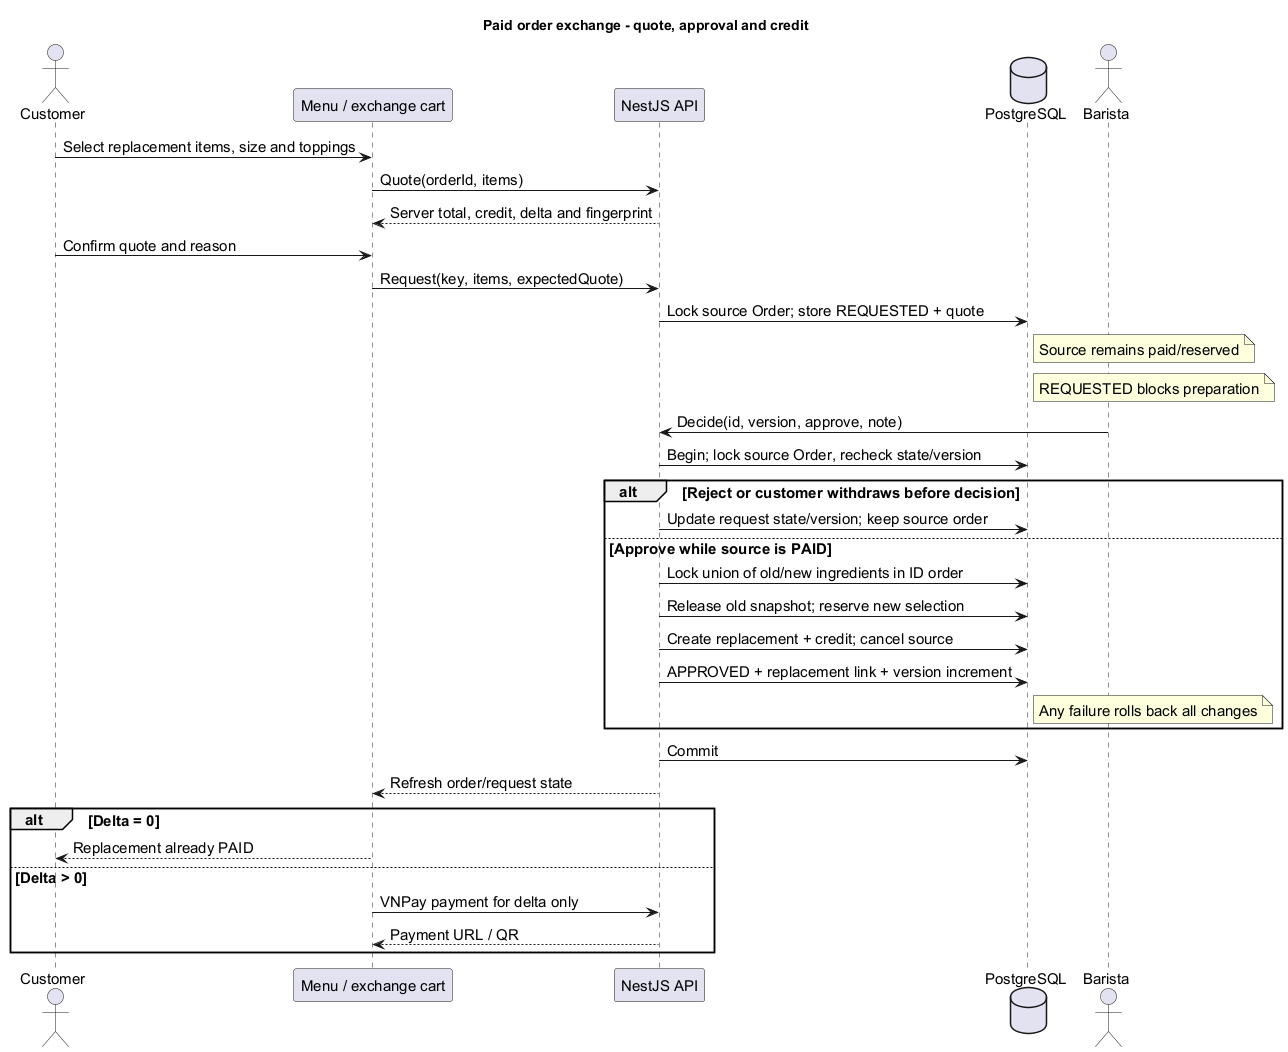
\includegraphics[width=\linewidth,height=.56\textheight,keepaspectratio]{assets/exchange/exchange-sequence.png}
\caption{Khách gửi yêu cầu, quầy quyết định, transaction thay đơn và thanh toán chênh lệch}
\end{figure}
